\section{Background}
\label{sec:bg}

\begin{figure}[t]
\centering
\IfFileExists{figures/fig_ladder.pdf}{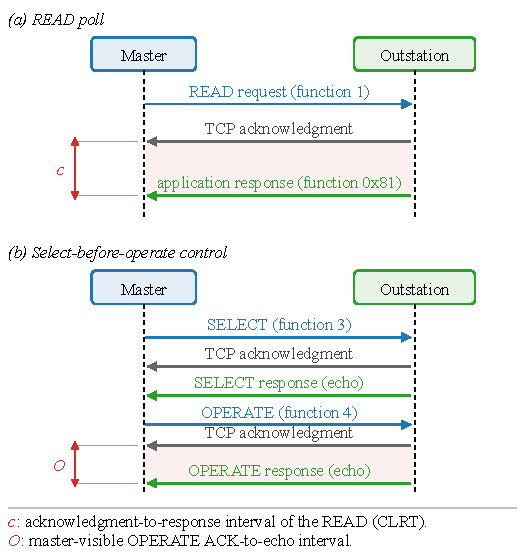
\includegraphics{figures/fig_ladder}}{\figplaceholder{DNP3 transaction ladder. Read (left): request, transport-layer acknowledgment, application-layer response, confirm. Select-before-Operate control (right): SELECT, acknowledgment, echo, OPERATE, acknowledgment, operate response. Mark the acknowledgment-to-response interval of the read and the operate-to-response interval of the control.}}
\caption{DNP3 transactions on the SEL-751. A read is a request, a transport-layer acknowledgment, and
an application-layer response; a Select-before-Operate control adds an OPERATE and its response. The
adversary times the acknowledgment-to-response interval of the read and the operate-to-response
interval of the control.}
\label{fig:ladder}
\end{figure}

\textbf{DNP3 polling and control.} DNP3 carries SCADA reads and controls over TCP between a master and
an outstation~\cite{ieeeIEEEStandardElectric2012}. The master periodically polls the outstation with a read request, and
the outstation returns the requested measurements in a response. A control uses Select-before-Operate:
the master sends a SELECT that names an output point, the outstation echoes it, and the master then
sends an OPERATE that actuates the point, which the outstation confirms. Figure~\ref{fig:ladder} shows
both exchanges.

\textbf{Cross-layer timing on a separate-acknowledgment device.} Our outstation is a physical SEL-751
feeder-protection relay. Because TCP acknowledges a request at the transport layer before the
application response is ready, each transaction exposes two events to an on-path observer: the
acknowledgment and, later, the response. Consequently, a read exposes the interval between its
acknowledgment and its response, and a control OPERATE exposes the interval between its request and its
operate response. These two intervals reflect the outstation's internal processing rather than the
network path, and they are the timing features the adversary uses (Section~\ref{sec:threat}).

\textbf{Programmable data planes.} Modern switches expose a match-action pipeline, programmable in P4,
that parses headers, keeps per-packet state, and holds packets in output queues at line rate. Since
this pipeline can delay and release a packet without a host in the loop, it is where \sysname runs,
changing no endpoint and no DNP3 byte.
